% Provenance (never printed): cycle 4 SVT, "La planete Terre": earthquakes,
% faults, seismic waves and their recording, magnitude and intensity, the
% link with plate boundaries; natural hazards (tsunamis) and prevention; see
% sources/book1/PROVENANCE.md. Book 1, grade 7, chapter 3.
% Vocabulary guard: P and S waves are named in prose only (they were named in
% g6.4, defined in Book 2 g11); "sediment" not before g7.4; "intensity" is
% always the earthquake's (homograph with physics: linker STOP list).
\chapter{الزلازل}\label{ch:g7:earthquakes}

في صباح 26~ديسمبر 2004، تحت \omterm{def:g2:water-on-earth:ocean}{البحر} قبالة الطرف الشمالي الغربي لجزيرة
سومطرة في إندونيسيا، انكسرت \omterm{def:g3:stones-pebbles-sand:rock}{الصخور} على طول \omterm{def:g7:earthquakes:fault}{صدع}: كان ذلك من أكبر \omterm{def:g4:volcanoes-earthquakes-first-look:earthquake}{الزلازل}
التي قيست في التاريخ. وعلى \omterm{def:g1:landscapes-around-us:water}{ساحل} سومطرة القريب، ارتفع \omterm{def:g2:water-on-earth:ocean}{البحر} في أمواج
بلغ علوها \qty{51}{m}، اجتاحت اليابسة حتى مسافة \qty{5}{km}. وفي
الساعات التالية عبرت الأمواج \omterm{def:g2:water-on-earth:ocean}{المحيط} الهندي وضربت \omterm{def:g1:landscapes-around-us:water}{سواحل} خمسة عشر بلدًا،
حتى إفريقيا البعيدة. ومات نحو 230\,000 إنسان. ولم يكن في \omterm{def:g2:water-on-earth:ocean}{المحيط}
الهندي يومئذ أي نظام للإنذار.
% ledger: usgs:largest, nws:tsunami-2004

\begin{omfigure}
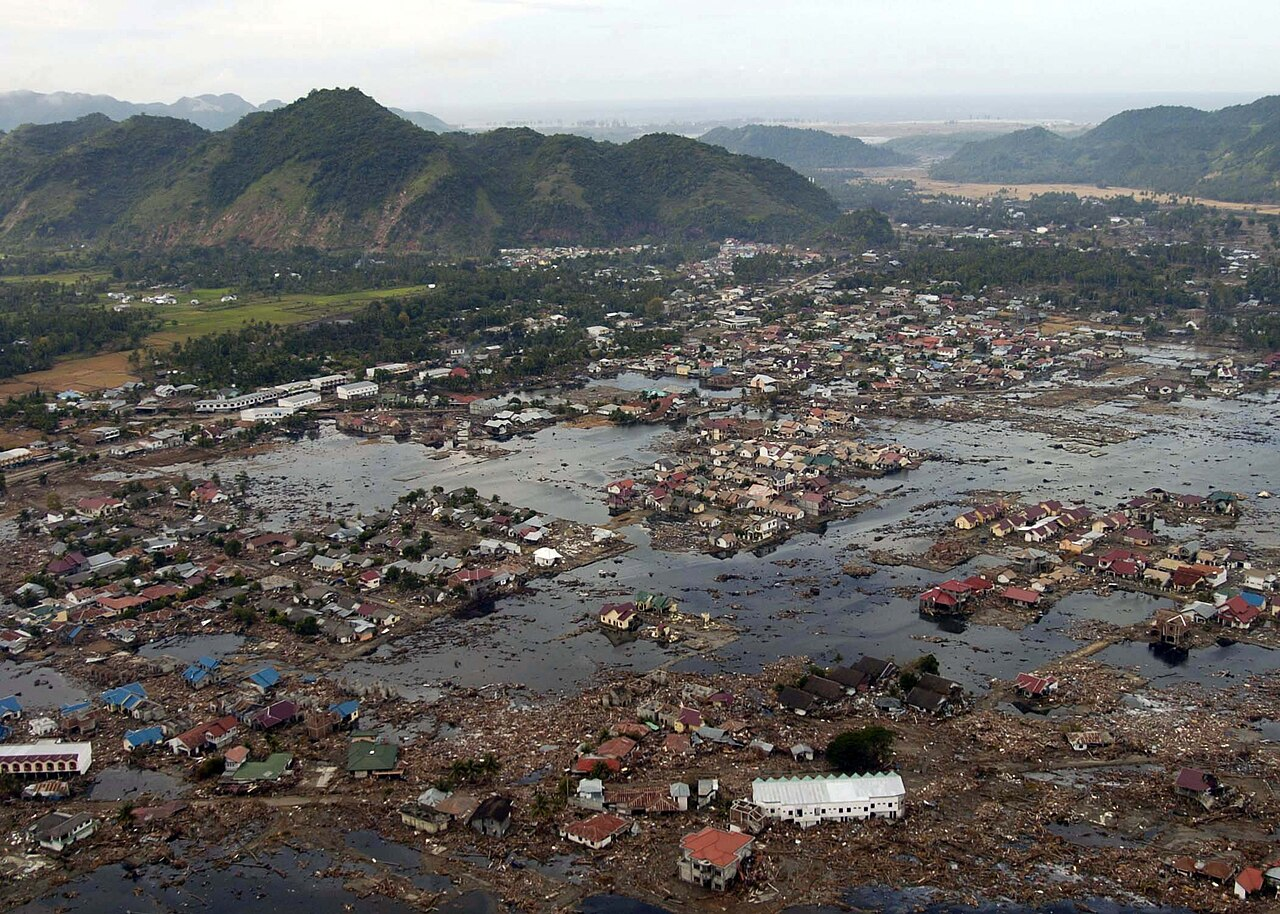
\includegraphics[width=0.78\linewidth]{images/book1/g7-tsunami-village.jpg}

{\small قرية قرب \omterm{def:g1:landscapes-around-us:water}{ساحل} سومطرة بعد أسبوع من \omterm{def:g7:earthquakes:tsunami}{تسونامي} 26~ديسمبر 2004. صورة
للبحرية الأمريكية التقطها فيليب~أ. ماكدانيال (ملك عام، عبر ويكيميديا
كومنز).}
% ledger: commons:tsunami-village
\label{fig:g7:earthquakes:tsunami-village}
\end{omfigure}

كيف تنكسر \omterm{def:g3:stones-pebbles-sand:rock}{الصخور}؟ وكيف يعرف العلماء، في غضون دقائق، أين ضرب \omterm{def:g4:volcanoes-earthquakes-first-look:earthquake}{الزلزال} وما
مقدار كبره؟ ولماذا ارتفع \omterm{def:g2:water-on-earth:ocean}{البحر}، بعد ساعات، على \omterm{def:g1:landscapes-around-us:water}{سواحل} لم يشعر فيها أحد
بأي شيء؟

\begin{recall}
\emph{\omterm{def:g4:volcanoes-earthquakes-first-look:earthquake}{الزلزال}} اهتزاز مفاجئ للأرض، تسببه \omterm{def:g3:stones-pebbles-sand:rock}{صخور} تنكسر وتنزلق في أعماق باطن
الأرض (\cref{ch:g4:volcanoes-earthquakes-first-look}). والغلاف الخارجي
للأرض مكوَّن من \omterm{def:g7:plate-tectonics:plate}{صفائح}، و92~\% من \omterm{def:g4:volcanoes-earthquakes-first-look:earthquake}{الزلازل} الكبيرة تقع على بعد أقل من
\qty{300}{km} من حد بين \omterm{def:g7:plate-tectonics:plate}{الصفائح} (\cref{ch:g7:plate-tectonics}). وحين
يضرب \omterm{def:g4:volcanoes-earthquakes-first-look:earthquake}{زلزال}، تنتشر أمواج عبر \omterm{def:g3:stones-pebbles-sand:rock}{صخور} الأرض كلها: نوع أسرع (الموجات P)
ونوع أبطأ (الموجات S)؛ وبقياس توقيت وصولها اكتشف العلماء \omterm{def:g6:inside-the-earth:layers}{اللب}
(\cref{ch:g6:inside-the-earth}).
\end{recall}

\section{صخور تنكسر}

تتحرك \omterm{def:g7:plate-tectonics:plate}{الصفائح} بضعة سنتيمترات في السنة، لكن حوافها خشنة: فهي تلتصق بعضها
ببعض بينما يواصل باقي \omterm{def:g7:plate-tectonics:plate}{الصفائح} حركته. فتنثني \omterm{def:g3:stones-pebbles-sand:rock}{الصخور} القريبة من الحافة
قليلًا، كمسطرة تضغطها من طرفيها، وتختزن طاقة. وحين يتغلب الدفع أخيرًا على
الاحتكاك، تنفك \omterm{def:g3:stones-pebbles-sand:rock}{الصخور} دفعة واحدة وتنزلق: وهذا الانزلاق المفاجئ هو \omterm{def:g4:volcanoes-earthquakes-first-look:earthquake}{الزلزال}.
% ledger: usgs:eq-basics

\begin{definition}[الصدع]\label{def:g7:earthquakes:fault}
\emph{الصدع}\index{صدع} كسر في \omterm{def:g3:stones-pebbles-sand:rock}{الصخور} تحرك على طوله الكتلتان الواقعتان على
جانبيه إحداهما بالنسبة إلى الأخرى. وأثناء \omterm{def:g4:volcanoes-earthquakes-first-look:earthquake}{الزلزال} تنزلق الكتلتان فجأة على
طول الصدع؛ وكلما كبر الصدع وكبر الانزلاق، كبر \omterm{def:g4:volcanoes-earthquakes-first-look:earthquake}{الزلزال}.
\end{definition}

يتكون \omterm{def:g7:plate-tectonics:plate-boundary}{حد الصفائح} من صدوع كثيرة، وعليها تقع معظم \omterm{def:g4:volcanoes-earthquakes-first-look:earthquake}{زلازل} العالم. لكن
الصدوع موجودة أيضًا داخل \omterm{def:g7:plate-tectonics:plate}{الصفائح}، وقد ينكسر بعضها هو الآخر. وحين ينكسر
\omterm{def:g7:earthquakes:fault}{صدع} كبير قرب السطح، يمكن أن يُرى الانزلاق على الأرض: درجة في حقل، أو طريق
مقطوع شطرين، أو سياج أو صف من الأشجار انزاح جانبًا.
% ledger: usgs:eq-basics

\begin{omfigure}
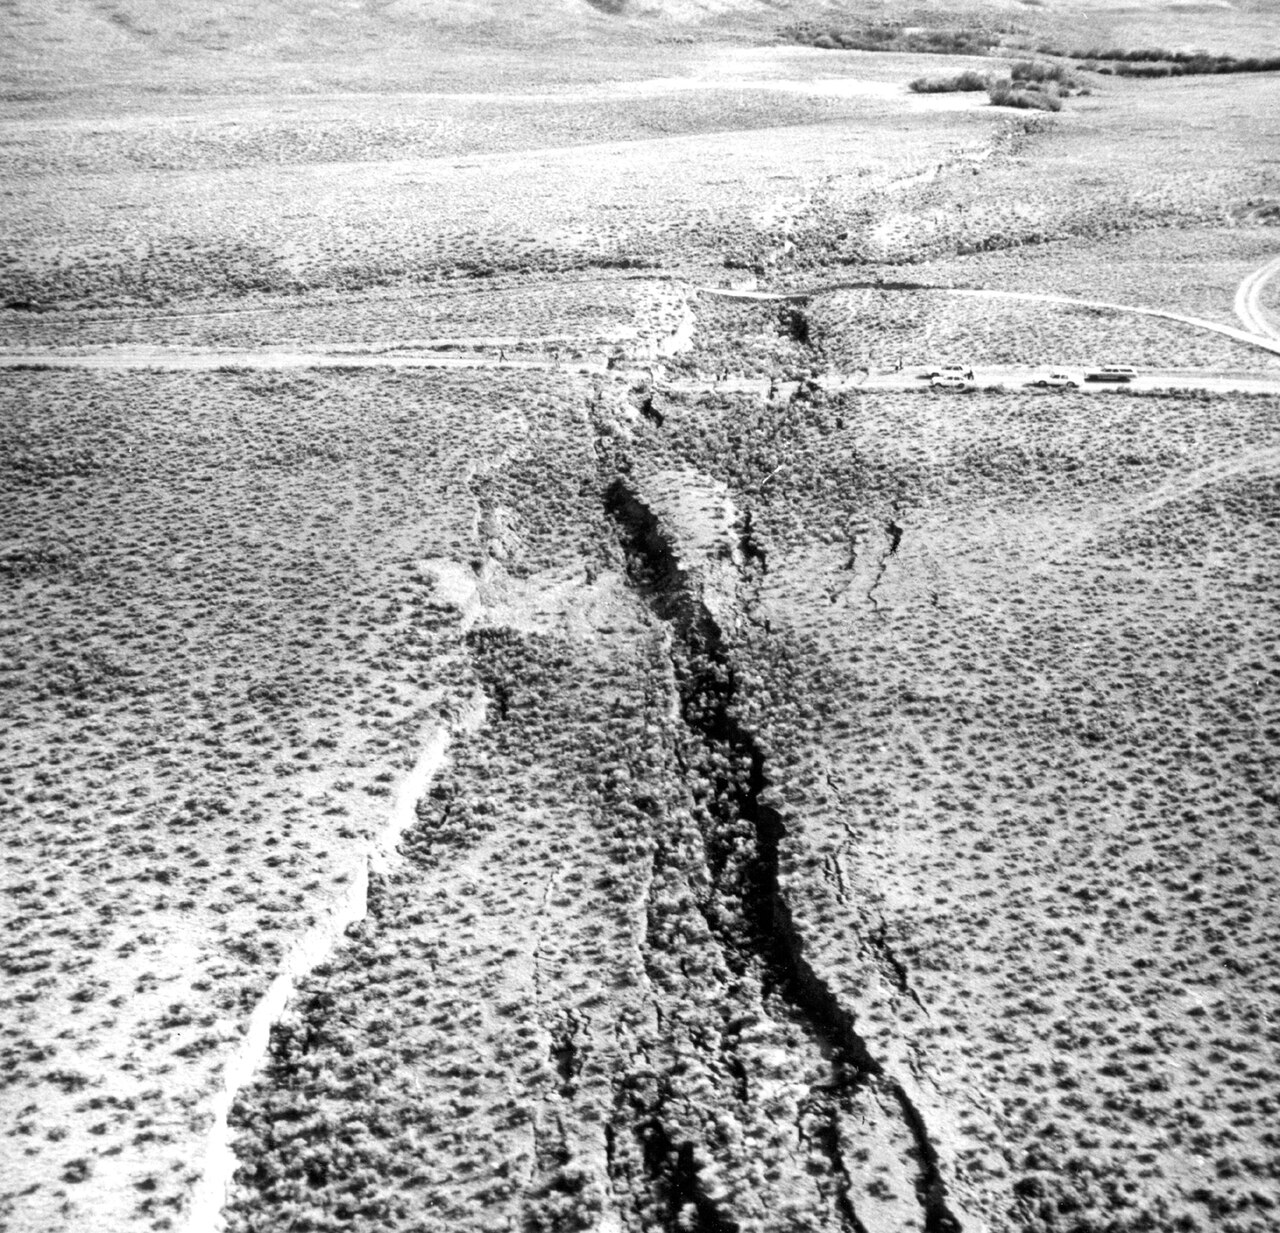
\includegraphics[width=0.62\linewidth]{images/book1/g7-borah-scarp.jpg}

{\small درجات في الأرض خلّفها \omterm{def:g4:volcanoes-earthquakes-first-look:earthquake}{زلزال} بوراه بيك عام 1983، في أيداهو
(الولايات المتحدة)، كما تُرى من الجو: على طول \omterm{def:g7:earthquakes:fault}{الصدع}، هبط أحد الجانبين
بالنسبة إلى الآخر، والدرجة تقطع الطريق في أعلى الصورة. الصورة:
ر.~إ. والاس، هيئة المسح الجيولوجي الأمريكية (ملك عام، عبر ويكيميديا
كومنز).}
% ledger: commons:borah-scarp
\label{fig:g7:earthquakes:borah}
\end{omfigure}

\begin{definition}[البؤرة والمركز السطحي]\label{def:g7:earthquakes:focus}
\emph{بؤرة}\index{بؤرة} \omterm{def:g4:volcanoes-earthquakes-first-look:earthquake}{الزلزال} هي المكان، تحت الأرض وعلى \omterm{def:g7:earthquakes:fault}{الصدع}، الذي يبدأ
منه الانزلاق. و\emph{المركز السطحي}\index{مركز سطحي} هو النقطة من سطح
الأرض الواقعة فوق البؤرة مباشرة.
\end{definition}

كثيرًا ما تكون \omterm{def:g7:earthquakes:focus}{البؤرة} على عمق بضعة كيلومترات إلى بضع عشرات من الكيلومترات.
فمن بين 7\,031 \omterm{def:g4:volcanoes-earthquakes-first-look:earthquake}{زلزالًا} \omterm{def:g7:earthquakes:magnitude}{قدرها}~6 أو أكثر سُجلت بين 1976 و2025، كانت \omterm{def:g7:earthquakes:focus}{بؤرة}
5\,561 منها --- أي 79~\% --- على عمق أقل من \qty{70}{km}. لكن 483 منها
بدأت على عمق يزيد على \qty{300}{km}، وأعمقها على عمق \qty{688}{km}: وهذه
\omterm{def:g4:volcanoes-earthquakes-first-look:earthquake}{الزلازل} العميقة تقع حيث تغوص \omterm{def:g7:plate-tectonics:plate}{صفيحة} تحت أخرى، داخل \omterm{def:g7:plate-tectonics:plate}{الصفيحة} الغائصة.
% ledger: data:usgs-comcat (figdata/grade-7/quake_counts.py, part depth)

نادرًا ما يأتي \omterm{def:g4:volcanoes-earthquakes-first-look:earthquake}{زلزال} كبير وحده. فكثيرًا ما تتبعه \omterm{def:g4:volcanoes-earthquakes-first-look:earthquake}{زلازل} أصغر في المكان نفسه،
هي \emph{الهزات الارتدادية}، أسابيع وشهورًا بل سنوات. وقد تسبقه أحيانًا
\omterm{def:g4:volcanoes-earthquakes-first-look:earthquake}{زلازل} أصغر، لكن لا أحد يستطيع أن يعرف أنها كانت إنذارات إلا بعد وقوع
\omterm{def:g4:volcanoes-earthquakes-first-look:earthquake}{الزلزال} الكبير: فالعلماء لا يستطيعون التنبؤ \omterm{def:g4:volcanoes-earthquakes-first-look:earthquake}{بالزلازل}. وكل ما يستطيعونه
أن يقولوا أي الصدوع ستنكسر من جديد يومًا ما، وأن يساعدوا الناس على
الاستعداد.
% ledger: usgs:eq-basics, usgs:seismograph

\begin{omfigure}
\begin{tikzpicture}[font=\small, x=1cm, y=1cm]
  % a block of crust seen in perspective: front face and top face
  \def\dx{2.2}\def\dy{1.3}
  % top surface: two blocks separated by the fault trace
  \fill[green!12] (0,0) -- (4.6,0) -- (4.6+\dx,\dy) -- (\dx,\dy) -- cycle;
  \fill[green!18] (4.6,0) -- (9,0) -- (9+\dx,\dy) -- (4.6+\dx,\dy) -- cycle;
  % front face
  \fill[brown!30] (0,0) -- (4.6,0) -- (3.4,-4) -- (0,-4) -- cycle;
  \fill[brown!40] (4.6,0) -- (9,0) -- (9,-4) -- (3.4,-4) -- cycle;
  % right face
  \fill[brown!22] (9,0) -- (9+\dx,\dy) -- (9+\dx,\dy-4) -- (9,-4) -- cycle;
  % fault plane on the front face and trace on top
  \draw[very thick, red!70!black] (4.6,0) -- (3.4,-4);
  \draw[very thick, red!70!black] (4.6,0) -- (4.6+\dx,\dy);
  % slip arrows
  \draw[-{Stealth[length=2.5mm]}, thick] (2.6,-0.35) -- (1.6,-0.35);
  \draw[-{Stealth[length=2.5mm]}, thick] (6.4,-0.35) -- (7.4,-0.35);
  \node[font=\footnotesize, anchor=south] at (2.1,-0.3) {\foreignlanguage{arabic}{الكتلة 1}};
  \node[font=\footnotesize, anchor=south] at (6.9,-0.3) {\foreignlanguage{arabic}{الكتلة 2}};
  % focus and waves
  \coordinate (F) at (3.95,-2.4);
  \foreach \r in {0.5,1.0,1.5,2.0}
    \draw[blue!60, dashed] (F) circle (\r);
  \fill[red!80!black] (F) circle (0.13);
  % epicentre: on the surface, straight above the focus (front edge of the top face)
  \coordinate (E) at (3.95,0);
  \draw[black!60, densely dotted, thick] (F) -- (E);
  \node[star, star points=5, star point ratio=2.4, fill=orange, draw=black, inner sep=1.4pt] at (E) {};
  % labels
  \node[anchor=west] at (9.5,-2.3) {البؤرة};
  \draw[black!60] (9.45,-2.3) -- (4.1,-2.4);
  \node[anchor=south west] at (4.9,1.9) {المركز السطحي};
  \draw[black!60] (4.95,1.95) -- (4.05,0.12);
  \node[anchor=south, red!70!black] at (6.8,1.3) {الصدع};
  \node[anchor=east, blue!60!black, align=right] at (-0.15,-2.6) {أمواج تنتشر\\في كل الاتجاهات};
  \draw[blue!60, -{Stealth}] (-0.1,-2.6) -- (1.9,-2.5);
\end{tikzpicture}

{\small \omterm{def:g7:earthquakes:fault}{صدع}، \omterm{def:g7:earthquakes:focus}{وبؤرة}، \omterm{def:g7:earthquakes:focus}{ومركز سطحي} (رسم، ليس بمقياس رسم). تنزلق الكتلتان
إحداهما بمحاذاة الأخرى على طول \omterm{def:g7:earthquakes:fault}{الصدع} (بالأحمر)؛ ويبدأ الانزلاق من
\omterm{def:g7:earthquakes:focus}{البؤرة}، وتنتشر منها أمواج في كل الاتجاهات، كالدوائر على سطح بركة.
\omterm{def:g7:earthquakes:focus}{والمركز السطحي} (النجمة) على السطح، فوق \omterm{def:g7:earthquakes:focus}{البؤرة} تمامًا.}
% ledger: usgs:eq-basics
\label{fig:g7:earthquakes:fault}
\end{omfigure}


\section{تسجيل الزلزال}

\begin{definition}[مقياس الزلازل والمخطط الزلزالي]\label{def:g7:earthquakes:seismometer}
\emph{مقياس الزلازل}\index{مقياس الزلازل} جهاز يسجل اهتزاز الأرض. وتسجيله،
وهو خط متعرج مرسوم بحسب الزمن، يسمى \emph{المخطط الزلزالي}\index{مخطط زلزالي}.
\end{definition}

فكرة \omterm{def:g7:earthquakes:seismometer}{مقياس الزلازل} بسيطة. إطار مثبت بإحكام في الأرض، يتدلى منه ثقل كبير
معلق بنابض. وحين تهتز الأرض، يهتز الإطار معها، لكن الثقل الكبير، الذي
لا يمسكه إلا نابضه، يبقى ساكنًا تقريبًا. ويسجل الجهاز حركة الإطار
بالنسبة إلى الثقل الساكن: وتلك هي حركة الأرض. وفي الرسم أدناه، يرسمها
قلم مثبت بالكتلة على ورق ملفوف حول أسطوانة دوّارة.
% ledger: usgs:seismograph

\begin{omfigure}
\begin{tikzpicture}[font=\small, x=1cm, y=1cm]
  \begin{scope}
    % ground
    \fill[brown!30] (-0.6,-0.6) rectangle (5.0,0);
    \draw[decorate, decoration={snake, amplitude=1.2pt, segment length=6pt}, brown!70!black, thick]
      (-0.6,0) -- (5.0,0);
    % frame
    \fill[black!55] (0,0) rectangle (0.25,3.2);
    \fill[black!55] (0,3.0) rectangle (2.4,3.25);
    % spring and weight
    \draw[decorate, decoration={coil, aspect=0.5, segment length=3pt, amplitude=4pt}, thick]
      (2.1,3.0) -- (2.1,2.1);
    \fill[black!80] (1.7,1.45) rectangle (2.5,2.1);
    \node[white, font=\scriptsize] at (2.1,1.78) {الكتلة};
    % pen arm and drum
    \draw[thick] (2.5,1.75) -- (3.45,1.75);
    \fill (3.45,1.75) circle (0.05);
    \draw[thick, fill=white] (3.95,1.75) circle (0.5);
    \draw[thick] (3.95,1.25) -- (3.95,0);
    \draw[-{Stealth}, black!60] (4.55,2.2) arc (40:-40:0.7);
    % labels
    \node[anchor=east, align=right, font=\footnotesize] at (-0.1,2.3) {إطار مثبت\\في الأرض};
    \node[anchor=west, font=\footnotesize] at (2.6,2.65) {نابض};
    \draw[black!60] (2.55,2.65) -- (2.25,2.6);
    \node[anchor=north, align=center, font=\footnotesize] at (2.1,1.35) {كتلة ثقيلة\\تبقى ساكنة};
    \node[anchor=west, align=left, font=\footnotesize] at (4.7,1.05) {أسطوانة دوّارة\\عليها ورق};
    \node[anchor=north, font=\footnotesize] at (2.2,-0.65) {الأرض تهتز};
  \end{scope}
  \begin{scope}[xshift=7.2cm, yshift=0.4cm]
    \begin{axis}[width=7.6cm, height=4.2cm, xmin=0, xmax=60, ymin=-1.1, ymax=1.1,
        axis x line=bottom, axis y line=none, xlabel={الزمن بالثواني},
        tick label style={font=\scriptsize}, label style={font=\footnotesize}, clip=false]
      \addplot[black, line width=0.4pt] table[x=t, y=v] {figdata/out/grade-7-epicentre-m-trace.dat};
      \draw[blue!70!black, -{Stealth[length=2mm]}] (axis cs:10,1.45) -- (axis cs:10,0.45);
      \node[blue!70!black, font=\scriptsize, anchor=south east] at (axis cs:10.5,1.45) {وصول الأمواج الأسرع};
      \draw[red!70!black, -{Stealth[length=2mm]}] (axis cs:20,1.45) -- (axis cs:20,1.05);
      \node[red!70!black, font=\scriptsize, anchor=south west] at (axis cs:19.5,1.45) {وصول الأمواج الأبطأ};
      \draw[{Stealth[length=2mm]}-{Stealth[length=2mm]}] (axis cs:10,-0.75) -- (axis cs:20,-0.75);
      \node[font=\scriptsize, anchor=east] at (axis cs:9,-0.75) {\foreignlanguage{arabic}{التأخر: 10 ثوانٍ}};
    \end{axis}
  \end{scope}
\end{tikzpicture}

{\small على اليسار: مبدأ \omterm{def:g7:earthquakes:seismometer}{مقياس الزلازل} (رسم). على اليمين: \omterm{def:g7:earthquakes:seismometer}{مخطط زلزالي}
رُسم لهذا الكتاب (ليس تسجيلًا حقيقيًا): الخط هادئ، ثم تصل الأمواج
الأسرع، ثم، بعد عشر ثوانٍ، الأمواج الأبطأ والأكبر.}
% ledger: usgs:seismograph (trace drawn by figdata/grade-7/epicentre.py, part m-trace)
\label{fig:g7:earthquakes:seismometer}
\end{omfigure}

\subsection*{على أي بعد كان الزلزال؟}

يخبرنا \omterm{def:g7:earthquakes:seismometer}{المخطط الزلزالي} بأكثر من «الأرض اهتزت». فالأمواج الأسرع تصل دائمًا
أولًا، والأبطأ بعدها. وقرب \omterm{def:g7:earthquakes:focus}{البؤرة} تصلان معًا تقريبًا؛ أما بعيدًا عنها
فتتأخر الأمواج الأبطأ أكثر فأكثر، تمامًا كما يتأخر الرعد عن البرق
أثناء \omterm{def:g5:natural-hazards:storm}{العاصفة} كلما كانت \omterm{def:g5:natural-hazards:storm}{العاصفة} أبعد. ولذلك فإن التأخر بين الوصولين
يدل على المسافة إلى \omterm{def:g4:volcanoes-earthquakes-first-look:earthquake}{الزلزال}.
% ledger: usgs:seismograph

كم كيلومترًا لكل ثانية من التأخر؟ ذلك يتوقف على سرعتي الموجتين في
\omterm{def:g3:stones-pebbles-sand:rock}{الصخور} التي تعبرانها. وبسرعات النموذج المرجعي للأرض
(\cref{ch:g6:inside-the-earth})، تعني كل ثانية من التأخر نحو \qty{7}{km}
في \omterm{def:g6:inside-the-earth:layers}{القشرة} العليا و\qty{9}{km} في \omterm{def:g6:inside-the-earth:layers}{القشرة} السفلى. وفي تمارين هذا الفصل
نستعمل القيمة المقرَّبة \qty{8}{km} لكل ثانية.
% ledger: data:prem (computed in figdata/grade-7/epicentre.py, part rule)

\begin{method}[إيجاد المركز السطحي بثلاث محطات]\label{met:g7:earthquakes:three-circles}
\begin{enumerate}
  \item اقرأ على \omterm{def:g7:earthquakes:seismometer}{المخطط الزلزالي} لكل محطة التأخر بين وصول الأمواج الأسرع
        ووصول الأمواج الأبطأ.
  \item حوّل كل تأخر إلى مسافة (هنا: $8 \times$ التأخر بالثواني، فتكون
        المسافة بالكيلومترات).
  \item على \omterm{def:g2:drawing-to-map:map}{الخريطة}، ارسم حول كل محطة دائرة نصف قطرها مسافتها. \omterm{def:g7:earthquakes:focus}{والمركز
        السطحي} يقع في مكان ما على كل دائرة.
  \item مع دائرتين، توجد عادة نقطتان ممكنتان؛ والدائرة الثالثة لا تمر إلا
        بإحداهما: تلك هي \omterm{def:g7:earthquakes:focus}{المركز السطحي}.
\end{enumerate}
\end{method}

\begin{example}[ثلاث دوائر]\label{ex:g7:earthquakes:three-circles}
تسجل ثلاث محطات \omterm{def:g4:volcanoes-earthquakes-first-look:earthquake}{الزلزال} نفسه. والتأخرات \qty{10}{s} في المحطة~M1،
و\qty{11.25}{s} في M2، و\qty{9.75}{s} في M3. فالمسافات هي
$8 \times 10 = \qty{80}{km}$ و$8 \times 11.25 = \qty{90}{km}$
و$8 \times 9.75 = \qty{78}{km}$. والدوائر الثلاث، المرسومة أدناه، تلتقي
في نقطة واحدة: \omterm{def:g7:earthquakes:focus}{المركز السطحي}.
% ledger: usgs:seismograph (figdata/grade-7/epicentre.py, parts m-stations and m-circles)
\end{example}

\begin{omfigure}
\begin{tikzpicture}
  \begin{axis}[axis equal image, width=8.2cm, xmin=-150, xmax=170, ymin=-160, ymax=160,
      xtick={-120,-80,...,160}, ytick={-120,-80,...,120}, grid=both, grid style={black!12},
      tick label style={font=\scriptsize}, xlabel={\babelsublr{km}}, ylabel={\babelsublr{km}}, label style={font=\footnotesize}]
    \addplot[blue!60!black, line width=0.6pt] table[x=x, y=y] {figdata/out/grade-7-epicentre-m-circles.dat};
    \addplot[only marks, mark=triangle*, mark size=3pt, black,
        nodes near coords, point meta=explicit symbolic,
        nodes near coords style={font=\scriptsize, anchor=north, yshift=-2pt}]
      table[x=x, y=y, meta=name] {figdata/out/grade-7-epicentre-m-stations.dat};
    \node[star, star points=5, star point ratio=2.4, fill=orange, draw=black, inner sep=1.6pt] at (axis cs:0,0) {};
    \draw[black!60] (axis cs:-4,-4) -- (axis cs:-60,-75);
    \node[font=\scriptsize, anchor=north east, inner sep=1pt] at (axis cs:-60,-75) {المركز السطحي};
  \end{axis}
\end{tikzpicture}

{\small كل دائرة مركزها محطة (مثلث)، ونصف قطرها يساوي بعد تلك المحطة عن
\omterm{def:g4:volcanoes-earthquakes-first-look:earthquake}{الزلزال}. والدوائر الثلاث لا تلتقي إلا في نقطة واحدة، هي \omterm{def:g7:earthquakes:focus}{المركز السطحي}
(النجمة).}
% ledger: usgs:seismograph (figdata/grade-7/epicentre.py, parts m-stations and m-circles)
\label{fig:g7:earthquakes:three-circles}
\end{omfigure}

\begin{omfigure}
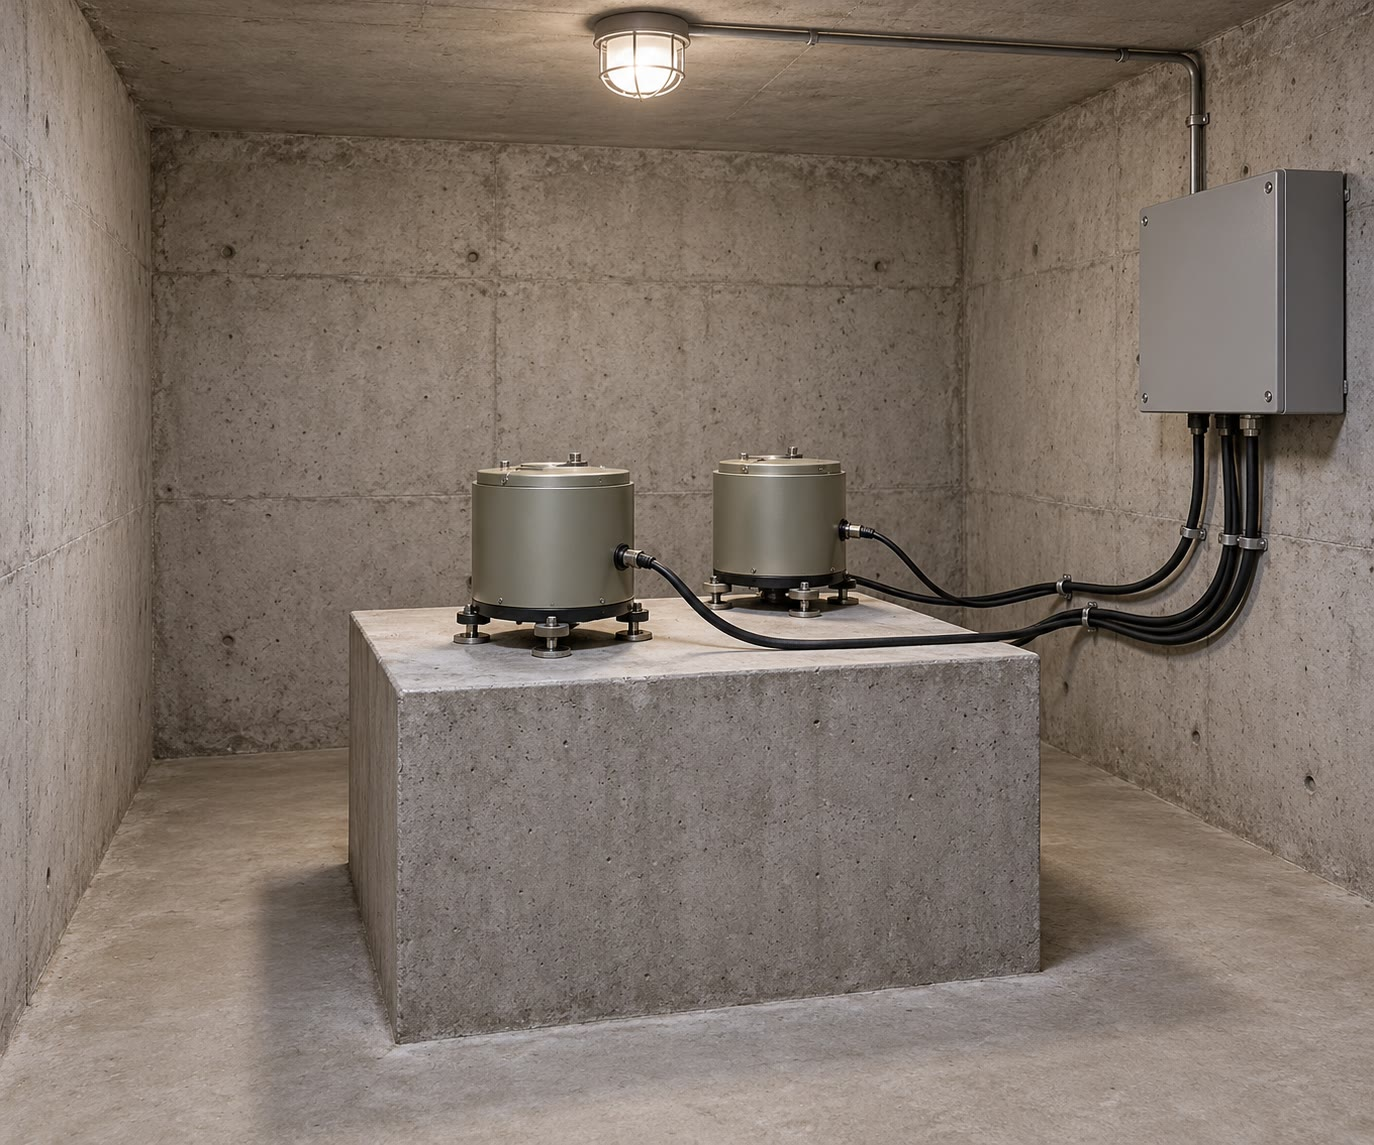
\includegraphics[width=0.58\linewidth]{images/book1/ai/g7-seismometer-vault.jpg}

{\small مقاييس \omterm{def:g4:volcanoes-earthquakes-first-look:earthquake}{زلازل} في غرفة هادئة تحت الأرض، موضوعة على قاعدة من الخرسانة
ترتكز على \omterm{def:g3:stones-pebbles-sand:rock}{الصخر}، بعيدًا عن الطرق والآلات (رسم توضيحي مولَّد بالذكاء
الاصطناعي لمشهد عام).}
\label{fig:g7:earthquakes:vault}
\end{omfigure}

\section{ما مقدار كبره؟ القدر والشدة}

يصف الزلزالَ عددان مختلفان، وكثيرًا ما يُخلط بينهما.

\begin{definition}[القدر]\label{def:g7:earthquakes:magnitude}
\emph{قدر}\index{قدر} \omterm{def:g4:volcanoes-earthquakes-first-look:earthquake}{الزلزال} يقيس حجمه: أي الطاقة المتحررة عند منشئه.
ويُحسب من المخططات الزلزالية. ولكل \omterm{def:g4:volcanoes-earthquakes-first-look:earthquake}{زلزال} قدر واحد، يُكتب برقم عشري
واحد، مثل 6.3 أو 9.1.
\end{definition}

\begin{definition}[الشدة]\label{def:g7:earthquakes:intensity}
\emph{شدة}\index{شدة} \omterm{def:g4:volcanoes-earthquakes-first-look:earthquake}{الزلزال} في مكان ما تصف مدى قوة اهتزاز الأرض هناك،
انطلاقًا مما شعر به الناس ومن الأضرار التي رأوها. وتُكتب بالأرقام
الرومانية، من I (لا يُشعر به) إلى XII (دمار شامل). وللزلزال الواحد
شدات كثيرة: شدة مختلفة في كل مكان.
\end{definition}

يرتفع سلم \omterm{def:g7:earthquakes:magnitude}{القدر} بسرعة. فكل درجة واحدة من \omterm{def:g7:earthquakes:magnitude}{القدر} تعني أمواجًا أكبر بنحو
10~مرات على \omterm{def:g7:earthquakes:seismometer}{المخطط الزلزالي}، وطاقة متحررة أكبر بنحو 32~مرة. \omterm{def:g4:volcanoes-earthquakes-first-look:earthquake}{والزلزال} الذي
\omterm{def:g7:earthquakes:magnitude}{قدره}~8 يحرر طاقة أكبر بنحو $32 \times 32 \approx 1000$ مرة من \omterm{def:g4:volcanoes-earthquakes-first-look:earthquake}{الزلزال} الذي
\omterm{def:g7:earthquakes:magnitude}{قدره}~6.
% ledger: usgs:mag-energy

\begin{method}[المقارنة بين قدرين]\label{met:g7:earthquakes:magnitudes}
للمقارنة بين طاقتي زلزالين، عُدّ الدرجات الكاملة بين قدريهما، واضرب
في 32 مرة لكل درجة: درجة واحدة، 32~مرة؛ درجتان، نحو 1000~مرة؛ ثلاث
درجات، نحو 32\,000~مرة.
\end{method}

\begin{example}[القدر 9 والقدر 7]\label{ex:g7:earthquakes:nine-seven}
كان \omterm{def:g7:earthquakes:magnitude}{قدر} \omterm{def:g4:volcanoes-earthquakes-first-look:earthquake}{زلزال} 2004 قبالة سومطرة 9.1. \omterm{def:g4:volcanoes-earthquakes-first-look:earthquake}{والزلزال} الذي \omterm{def:g7:earthquakes:magnitude}{قدره}~7.1 أصغر منه
بدرجتين: فقد حرر طاقة أقل بنحو $32 \times 32 = 1024$ مرة، أي نحو
1000~مرة.
% ledger: usgs:largest, usgs:mag-energy
\end{example}

أكبر \omterm{def:g4:volcanoes-earthquakes-first-look:earthquake}{الزلازل} التي قيست في التاريخ وقعت كلها حيث تغوص \omterm{def:g7:plate-tectonics:plate}{صفيحة} تحت أخرى:
\omterm{def:g7:earthquakes:magnitude}{القدر}~9.5 في تشيلي في 22~مايو 1960، و9.2 في ألاسكا عام 1964، و9.1 قبالة
سومطرة عام 2004، و9.1 قبالة \omterm{def:g1:landscapes-around-us:water}{ساحل} اليابان في 11~مارس 2011. \omterm{def:g4:volcanoes-earthquakes-first-look:earthquake}{والزلازل} الكبيرة
نادرة، وكلما كبرت ازدادت ندرة، كما يبين المخطط: فمع كل درجة صعودًا في
\omterm{def:g7:earthquakes:magnitude}{القدر}، يقل عددها نحو عشر مرات.
% ledger: usgs:largest, data:usgs-comcat

\begin{omfigure}
\begin{tikzpicture}
  \begin{axis}[ybar, width=0.72\linewidth, height=5.4cm, bar width=22pt,
      ymode=log, log origin y=infty, ymin=0.01, ymax=600,
      xtick=data, xticklabels={{\foreignlanguage{arabic}{من 6 إلى 6.9}}, {\foreignlanguage{arabic}{من 7 إلى 7.9}}, {\foreignlanguage{arabic}{من 8 إلى 8.9}}, {\foreignlanguage{arabic}{9 أو أكثر}}},
      xlabel={القدر}, ylabel={عدد الزلازل في السنة},
      ytick={0.01,0.1,1,10,100}, yticklabels={0.01,0.1,1,10,100},
      tick label style={font=\scriptsize}, label style={font=\small},
      nodes near coords, point meta=explicit symbolic,
      nodes near coords style={font=\scriptsize}, enlarge x limits=0.18,
      axis x line*=bottom, axis y line*=left]
    \addplot[fill=omThm!45, draw=omThm!80!black] table[x=cls, y=per_year, meta=per_year] {figdata/out/grade-7-quake_counts.dat};
  \end{axis}
\end{tikzpicture}

{\small عدد \omterm{def:g4:volcanoes-earthquakes-first-look:earthquake}{الزلازل} في السنة، في المتوسط على مدى 1976--2025، بحسب \omterm{def:g7:earthquakes:magnitude}{القدر}.
والسلم الرأسي خاص: كل خط فيه يساوي عشرة أضعاف الخط الذي تحته.
البيانات: فهرس \omterm{def:g4:volcanoes-earthquakes-first-look:earthquake}{الزلازل} لهيئة المسح الجيولوجي الأمريكية (7\,031 \omterm{def:g4:volcanoes-earthquakes-first-look:earthquake}{زلزالًا}
\omterm{def:g7:earthquakes:magnitude}{قدرها}~6 أو أكثر).}
% ledger: data:usgs-comcat (figdata/grade-7/quake_counts.py, main table)
\label{fig:g7:earthquakes:counts}
\end{omfigure}

ليس لسلم \omterm{def:g7:earthquakes:intensity}{الشدة} صيغة رياضية: إنه قائمة بما يحدث. ويعرضه الجدول في
صيغة مختصرة.
% ledger: usgs:mmi, usgs:mmi-page

\begin{center}
\small
\begin{tabular}{|c|p{0.8\linewidth}|}
\hline
\textbf{\omterm{def:g7:earthquakes:intensity}{الشدة}} & \textbf{ما يُشعر به وما يُرى} \\
\hline
I & لا يُشعر به، إلا عند قلة قليلة جدًا من الناس \\
II & لا يشعر به إلا قليل من الناس وهم في راحة، ولا سيما في الطوابق العليا؛ وقد تتأرجح الأشياء المعلقة \\
III & يُشعر به داخل البيوت؛ ويشبه مرور شاحنة \\
IV & يشعر به كثيرون داخل البيوت؛ وتهتز الأطباق والنوافذ والأبواب \\
V & يشعر به كل الناس تقريبًا، ويستيقظ كثيرون؛ وتنكسر بعض الأطباق والنوافذ \\
VI & يشعر به الجميع، ويفزع كثيرون؛ ويتحرك بعض الأثاث الثقيل؛ وأضرار طفيفة \\
VII & أضرار قليلة في المباني المتينة البناء، وكثيرة في الرديئة البناء؛ وتنكسر بعض المداخن \\
VIII & أضرار كبيرة في المباني العادية، وينهار بعضها جزئيًا؛ وتسقط المداخن والجدران \\
IX & أضرار جسيمة حتى في المباني المتينة؛ وتنزاح المباني عن أساساتها \\
X & تُدمَّر معظم المباني مع أساساتها؛ وتلتوي القضبان الحديدية \\
XI & لا يبقى قائمًا إلا قليل من المباني؛ وتُدمَّر الجسور \\
XII & دمار شامل؛ وتُقذف الأشياء في الهواء \\
\hline
\end{tabular}
\end{center}
% ledger: usgs:mmi

تكون \omterm{def:g7:earthquakes:intensity}{الشدة} عادة أعلى ما تكون قرب \omterm{def:g7:earthquakes:focus}{المركز السطحي}، وتتناقص مع المسافة. لكنها
تتوقف أيضًا على الأرض: \omterm{def:g3:stones-pebbles-sand:rock}{فالصخر} الصلب هو الأقل اهتزازًا، \omterm{def:g3:stones-pebbles-sand:sand}{والوحل} الطري هو
الأكثر. وقد تهتز مدينة مبنية على أرض طرية أشد من مدينة أخرى أقرب منها
إلى \omterm{def:g7:earthquakes:focus}{المركز السطحي} لكنها مبنية على \omterm{def:g3:stones-pebbles-sand:rock}{الصخر}.
% ledger: usgs:mag-energy

\begin{omfigure}
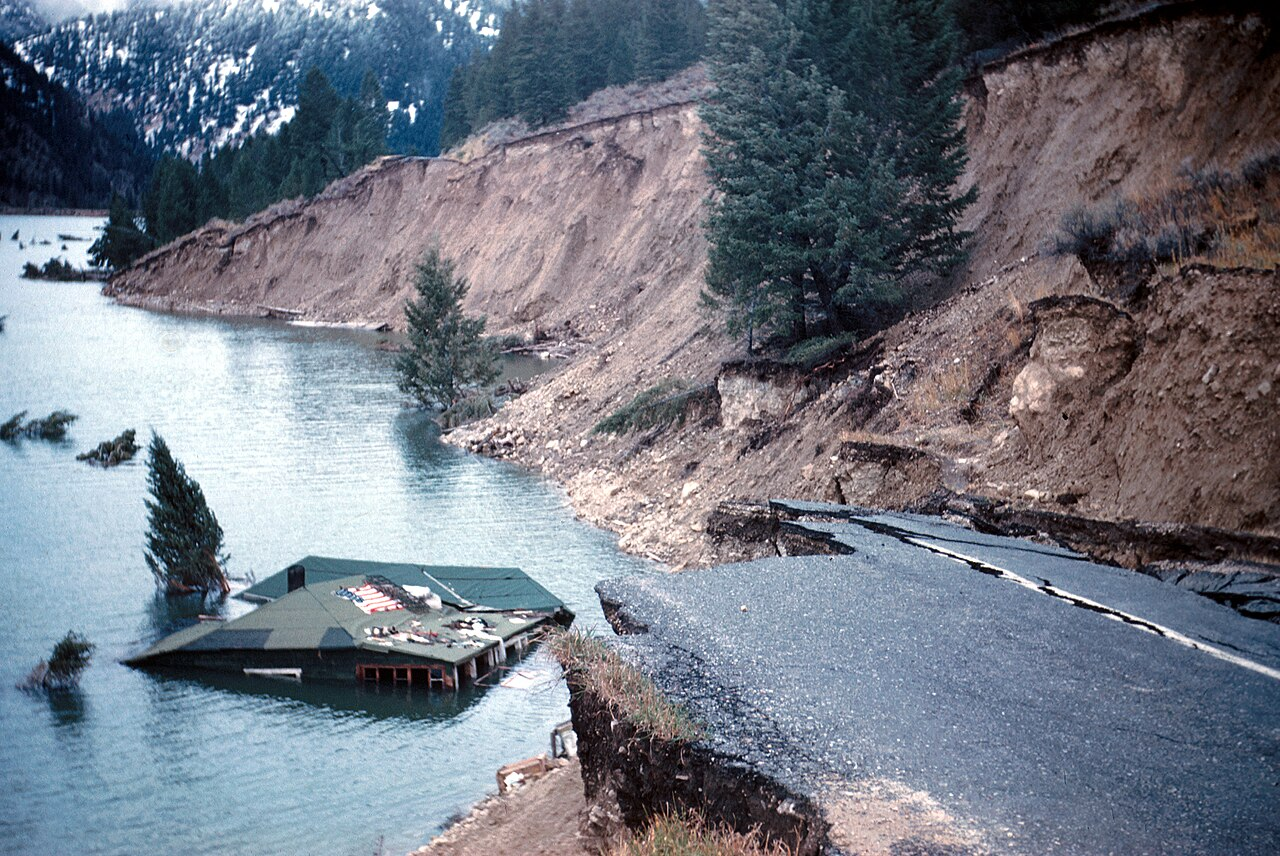
\includegraphics[width=0.6\linewidth]{images/book1/g7-hebgen-road.jpg}

{\small بعد \omterm{def:g4:volcanoes-earthquakes-first-look:earthquake}{زلزال} \omterm{def:g1:landscapes-around-us:water}{بحيرة} هيبغن، في مونتانا (الولايات المتحدة)، في أغسطس
1959: انزلق الطريق المحاذي \omterm{def:g1:landscapes-around-us:water}{للبحيرة} في الماء، وانتهى نُزُل إلى أن صار
مغمورًا بالماء تقريبًا. وأضرار كهذه علامة على \omterm{def:g7:earthquakes:intensity}{شدة} عالية. الصورة:
إ.~ج. ويتكايند، هيئة المسح الجيولوجي الأمريكية (ملك عام، عبر ويكيميديا
كومنز).}
% ledger: commons:hebgen-road, usgs:mmi
\label{fig:g7:earthquakes:hebgen}
\end{omfigure}

\section{التسونامي}

\begin{definition}[التسونامي]\label{def:g7:earthquakes:tsunami}
\emph{التسونامي}\index{تسونامي} سلسلة من أمواج \omterm{def:g2:water-on-earth:ocean}{البحر} تطلقها حركة مفاجئة
لقاع \omterm{def:g2:water-on-earth:ocean}{البحر} --- غالبًا \omterm{def:g4:volcanoes-earthquakes-first-look:earthquake}{زلزال} تحت \omterm{def:g2:water-on-earth:ocean}{البحر}، وأحيانًا \omterm{def:g4:volcanoes-earthquakes-first-look:eruption}{ثوران} بركاني --- ويمكنها
أن تعبر محيطات بأكملها وتغمر \omterm{def:g1:landscapes-around-us:water}{السواحل}.
\end{definition}

حين ينكسر \omterm{def:g7:earthquakes:fault}{صدع} تحت \omterm{def:g2:water-on-earth:ocean}{البحر}، يرتفع قاع \omterm{def:g2:water-on-earth:ocean}{البحر} أو ينخفض فجأة، فيرفع أو يخفض
عمود الماء كله الذي فوقه. فينتشر الماء في أمواج. وفي عرض \omterm{def:g2:water-on-earth:ocean}{المحيط} العميق،
يثير \omterm{def:g7:earthquakes:tsunami}{التسونامي} الدهشة: فنادرًا ما يزيد علوه على متر واحد، ولا تكاد السفن
تلاحظ مروره من تحتها. لكنه سريع: أكثر من \qty{800}{km/h}، بسرعة طائرة
نفاثة. وحين يبلغ المياه الضحلة قرب \omterm{def:g1:landscapes-around-us:water}{الساحل}، يتباطأ إلى 30 أو
\qty{50}{km/h} --- وهي سرعة لا يقدر أحد على الجري بمثلها --- ويزداد علوًا.
ويقل علو معظم أمواج \omterm{def:g7:earthquakes:tsunami}{التسونامي} عن \qty{3}{m} عند \omterm{def:g1:landscapes-around-us:water}{الساحل}؛ أما أكبرها فيتجاوز
\qty{30}{m}. والموجة الأولى ليست دائمًا الأكبر، وقد تظل الأمواج تتوالى
ساعات.
% ledger: nws:tsunami-speed, nws:tsunami-safety

\begin{omfigure}
\begin{tikzpicture}[font=\small, x=1cm, y=1cm]
  % sea floor profile: deep ocean on the left, shelf and coast on the right
  \fill[omSea!35] (0,0) -- (13.2,0) -- (13.2,-0.2) -- (11.4,-0.45) -- (10.2,-1.0) -- (8.8,-2.6) -- (0,-2.6) -- cycle;
  \fill[brown!35] (0,-2.6) -- (8.8,-2.6) -- (10.2,-1.0) -- (11.4,-0.45) -- (13.2,-0.2) -- (13.2,0.5) -- (14.2,1.0) -- (14.2,-3.3) -- (0,-3.3) -- cycle;
  % the broken fault under the sea, at left; one block lifted
  \draw[very thick, red!70!black] (1.9,-3.3) -- (2.3,-2.6);
  \draw[-{Stealth[length=2mm]}, thick] (2.75,-3.1) -- (2.75,-2.75);
  \node[anchor=north west, font=\footnotesize, red!70!black] at (0.1,-3.35) {ينكسر الصدع فيقفز قاع البحر};
  % wave: low and long in the deep ocean, short and tall near the coast
  \draw[blue!70!black, thick] (0,0) .. controls (1.2,0.18) and (2.2,0.18) .. (3.4,0)
     -- (5.0,0) .. controls (5.8,0.12) and (6.6,0.12) .. (7.4,0) -- (10.6,0)
     .. controls (11.0,0.55) and (11.6,0.9) .. (12.1,0) -- (13.2,0);
  \node[align=center, font=\footnotesize] at (2.0,0.85) {\foreignlanguage{arabic}{المحيط العميق: علوه نحو \babelsublr{1 m}،}\\\foreignlanguage{arabic}{وسرعته أكثر من \babelsublr{800 km/h}}};
  \node[align=center, font=\footnotesize] at (11.1,1.55) {\foreignlanguage{arabic}{قرب الساحل: أبطأ،}\\\foreignlanguage{arabic}{من \babelsublr{30} إلى \babelsublr{50 km/h}، وأعلى بكثير}};
  \draw[-{Stealth[length=2.5mm]}, thick, blue!70!black] (4.4,0.45) -- (6.4,0.45);
  \node[font=\footnotesize] at (6.0,-1.5) {عمق آلاف الأمتار};
  \node[font=\footnotesize] at (12.0,-0.75) {مياه ضحلة};
\end{tikzpicture}

{\small \omterm{def:g7:earthquakes:tsunami}{تسونامي} يعبر \omterm{def:g2:water-on-earth:ocean}{المحيط} (رسم، ليس بمقياس رسم: علو الموجة مبالغ فيه
كثيرًا). إنه منخفض وسريع جدًا فوق \omterm{def:g2:water-on-earth:ocean}{المحيط} العميق؛ ويتباطأ ويعلو في
المياه الضحلة قرب \omterm{def:g1:landscapes-around-us:water}{الساحل}.}
% ledger: nws:tsunami-speed
\label{fig:g7:earthquakes:tsunami}
\end{omfigure}

\begin{example}[من سومطرة إلى سريلانكا]\label{ex:g7:earthquakes:colombo}
تبعد كولومبو، كبرى مدن سريلانكا، نحو \qty{1830}{km} عن \omterm{def:g7:earthquakes:focus}{المركز السطحي} \omterm{def:g4:volcanoes-earthquakes-first-look:earthquake}{لزلزال}
2004. وبسرعة \qty{800}{km/h}، يقطع \omterm{def:g7:earthquakes:tsunami}{التسونامي} هذه المسافة في
$1830 \div 800 \approx 2.3$~ساعة، أي نحو ساعتين و17~دقيقة. ولم يشعر أحد
في سريلانكا \omterm{def:g4:volcanoes-earthquakes-first-look:earthquake}{بالزلزال}: فقد جاءت الموجة دون أي إنذار سوى \omterm{def:g2:water-on-earth:ocean}{البحر} نفسه.
% ledger: nws:tsunami-speed, usgs:largest (distance and time in figdata/grade-7/quake_counts.py, part tsunami)
\end{example}

\begin{remark}[الإنذار الذي يعطيه البحر]\label{rem:g7:earthquakes:natural-warning}
% ledger: nws:tsunami-natural-warning, nws:tsunami-speed, shakeout:dch
على \omterm{def:g1:landscapes-around-us:water}{الساحل}، قد تنبئ ثلاث علامات \omterm{def:g7:earthquakes:tsunami}{بتسونامي}: \omterm{def:g4:volcanoes-earthquakes-first-look:earthquake}{زلزال} قوي أو طويل؛ أو \omterm{def:g2:water-on-earth:ocean}{بحر} يتصرف
على نحو غريب --- \omterm{def:g5:water-shapes-the-land:flood}{فيضان} مفاجئ، أو ماء ينحسر بعيدًا عن الشاطئ فيكشف قاع
\omterm{def:g2:water-on-earth:ocean}{البحر} كجزر شديد الانخفاض؛ أو هدير عالٍ يأتي من \omterm{def:g2:water-on-earth:ocean}{المحيط}. وأثناء الاهتزاز،
احمِ نفسك كما تعلمت (انبطح، واحتمِ، وتمسّك). ثم لا تنتظر إنذارًا رسميًا:
اصعد إلى أعلى ما تستطيع، أو ابتعد في اليابسة قدر ما تستطيع، في الحال.
\omterm{def:g7:earthquakes:tsunami}{فالتسونامي} الآتي من \omterm{def:g4:volcanoes-earthquakes-first-look:earthquake}{زلزال} قريب قد يصل في غضون دقائق.
\end{remark}


\section{تمارين}

\begin{exercise}[$\star$]\label{exo:g7:earthquakes:1}
صِل كل كلمة بمعناها: \omterm{def:g7:earthquakes:fault}{الصدع}؛ \omterm{def:g7:earthquakes:focus}{البؤرة}؛ \omterm{def:g7:earthquakes:focus}{المركز السطحي}؛ \omterm{def:g7:earthquakes:seismometer}{مقياس الزلازل}؛ \omterm{def:g7:earthquakes:magnitude}{القدر}؛
\omterm{def:g7:earthquakes:intensity}{الشدة}. (أ) المكان تحت الأرض الذي يبدأ منه الانزلاق. (ب) مدى قوة اهتزاز
الأرض في مكان واحد. (ج) كسر في \omterm{def:g3:stones-pebbles-sand:rock}{الصخور} تحرك على طوله الجانبان. (د) النقطة
من السطح الواقعة فوق \omterm{def:g7:earthquakes:focus}{البؤرة}. (ه) حجم \omterm{def:g4:volcanoes-earthquakes-first-look:earthquake}{الزلزال}، وهو عدد واحد لكل \omterm{def:g4:volcanoes-earthquakes-first-look:earthquake}{زلزال}.
(و) جهاز يسجل اهتزاز الأرض.
\end{exercise}

\begin{exercise}[$\star$]\label{exo:g7:earthquakes:2}
تقع \omterm{def:g7:earthquakes:focus}{بؤرة} \omterm{def:g4:volcanoes-earthquakes-first-look:earthquake}{زلزال} على عمق \qty{30}{km} تحت قرية مباشرة. (أ) أين \omterm{def:g7:earthquakes:focus}{المركز
السطحي}؟ (ب) كم تبعد القرية عن \omterm{def:g7:earthquakes:focus}{البؤرة}؟ (ج) تبعد قرية ثانية \qty{40}{km} عن
\omterm{def:g7:earthquakes:focus}{المركز السطحي}. هل تكون \omterm{def:g7:earthquakes:intensity}{الشدة} فيها عادة أعلى أم أدنى منها في القرية الأولى؟
لماذا؟
\end{exercise}

\begin{exercise}[$\star$]\label{exo:g7:earthquakes:3}
\omterm{def:g7:earthquakes:magnitude}{قدر} أم \omterm{def:g7:earthquakes:intensity}{شدة}؟ (أ) «بلغ \omterm{def:g4:volcanoes-earthquakes-first-look:earthquake}{الزلزال} 6.8». (ب) «في شارعنا سقطت كل الأطباق
وانكسرت مدخنة». (ج) «كانت VI في المدينة وIV في قرى \omterm{def:g1:landscapes-around-us:landform}{التلال}». (د) «حرّر
طاقة أكبر 32~مرة من طاقة \omterm{def:g4:volcanoes-earthquakes-first-look:earthquake}{زلزال} العام الماضي».
\end{exercise}

\begin{exercise}[$\star$]\label{exo:g7:earthquakes:4}
صواب أم خطأ؟ صحّح العبارات الخاطئة. (أ) يستطيع العلماء أن يعرفوا قبل أسبوع
متى سيضرب \omterm{def:g4:volcanoes-earthquakes-first-look:earthquake}{زلزال}. (ب) في عرض \omterm{def:g2:water-on-earth:ocean}{المحيط}، \omterm{def:g7:earthquakes:tsunami}{التسونامي} جدار هائل من الماء. (ج)
\omterm{def:g4:volcanoes-earthquakes-first-look:earthquake}{للزلزال} الواحد \omterm{def:g7:earthquakes:magnitude}{قدر} واحد لكن شدات كثيرة. (د) معظم \omterm{def:g4:volcanoes-earthquakes-first-look:earthquake}{الزلازل} الكبيرة تقع قرب
\omterm{def:g7:plate-tectonics:plate-boundary}{حدود الصفائح}.
\end{exercise}

\begin{exercise}[$\star\star$]\label{exo:g7:earthquakes:5}
استعمل مخطط عدد \omterm{def:g4:volcanoes-earthquakes-first-look:earthquake}{الزلازل} في السنة. (أ) كم \omterm{def:g4:volcanoes-earthquakes-first-look:earthquake}{زلزالًا} \omterm{def:g7:earthquakes:magnitude}{قدره} من 6 إلى 6.9 يقع
تقريبًا في السنة؟ وكم \omterm{def:g4:volcanoes-earthquakes-first-look:earthquake}{زلزالًا} \omterm{def:g7:earthquakes:magnitude}{قدره} من 7 إلى 7.9؟ (ب) كم مرة يقل عدد الثانية
عن عدد الأولى؟ (ج) اجمع الأعمدة الثلاثة ابتداء من 7: كم \omterm{def:g4:volcanoes-earthquakes-first-look:earthquake}{زلزالًا} \omterm{def:g7:earthquakes:magnitude}{قدره} 7 أو
أكثر يقع تقريبًا في السنة؟ (د) يذكر المخطط 0.04 في السنة \omterm{def:g7:earthquakes:magnitude}{للقدر} 9 أو
أكثر. فكم يكون ذلك في 50~سنة؟
\end{exercise}

\begin{exercise}[$\star\star$]\label{exo:g7:earthquakes:6}
استعمل طريقة المقارنة بين \omterm{def:g7:earthquakes:magnitude}{قدرين}. (أ) كم مرة تزيد الطاقة التي يحررها \omterm{def:g4:volcanoes-earthquakes-first-look:earthquake}{زلزال}
\omterm{def:g7:earthquakes:magnitude}{قدره} 7 على طاقة \omterm{def:g4:volcanoes-earthquakes-first-look:earthquake}{زلزال} \omterm{def:g7:earthquakes:magnitude}{قدره} 6؟ (ب) \omterm{def:g4:volcanoes-earthquakes-first-look:earthquake}{وزلزال} \omterm{def:g7:earthquakes:magnitude}{قدره} 8 على \omterm{def:g4:volcanoes-earthquakes-first-look:earthquake}{زلزال} \omterm{def:g7:earthquakes:magnitude}{قدره} 6؟ (ج) كم
مرة تكبر أمواجه على \omterm{def:g7:earthquakes:seismometer}{المخطط الزلزالي}، على المسافة نفسها، بين \omterm{def:g7:earthquakes:magnitude}{القدر} 6
\omterm{def:g7:earthquakes:magnitude}{والقدر} 8؟
\end{exercise}

\begin{exercise}[$\star\star$]\label{exo:g7:earthquakes:7}
استعمل \qty{8}{km} لكل ثانية من التأخر بين الأمواج الأسرع والأمواج
الأبطأ. (أ) تسجل محطة تأخرًا قدره \qty{5}{s}. على أي بعد كان \omterm{def:g4:volcanoes-earthquakes-first-look:earthquake}{الزلزال}؟ (ب)
وتسجل محطة أخرى \qty{25}{s}. (ج) ضرب \omterm{def:g4:volcanoes-earthquakes-first-look:earthquake}{زلزال} على بعد \qty{120}{km} من
محطة: ما التأخر الذي ستقرؤه المحطة؟ (د) لماذا لا تستطيع محطة واحدة وحدها
أن تحدد مكان \omterm{def:g7:earthquakes:focus}{المركز السطحي}؟
\end{exercise}

\begin{exercise}[$\star\star$]\label{exo:g7:earthquakes:8}
استعمل جدول \omterm{def:g7:earthquakes:intensity}{الشدة}. أعطِ \omterm{def:g7:earthquakes:intensity}{الشدة} لكل بلاغ. (أ) «شعر به الجميع تقريبًا؛
استيقظنا وانكسر كوبان». (ب) «لم تشعر به إلا جدتي، وهي مستريحة في الطابق
العلوي؛ وتأرجح المصباح». (ج) «سقطت الجدران والمداخن؛ وانهارت عدة بيوت
جزئيًا». (د) أعطى \omterm{def:g4:volcanoes-earthquakes-first-look:earthquake}{الزلزال} نفسه البلاغين (أ) و(ج). اشرح كيف يكون ذلك
ممكنًا.
\end{exercise}

\begin{exercise}[$\star\star$]\label{exo:g7:earthquakes:9}
من بين \omterm{def:g4:volcanoes-earthquakes-first-look:earthquake}{الزلازل} التي \omterm{def:g7:earthquakes:magnitude}{قدرها}~6 أو أكثر في 1976--2025، وعددها 7\,031، كانت
\omterm{def:g7:earthquakes:focus}{بؤرة} 5\,561 منها على عمق أقل من \qty{70}{km}. (أ) كم \omterm{def:g4:volcanoes-earthquakes-first-look:earthquake}{زلزالًا} كانت بؤرته
أعمق؟ (ب) ما النسبة المئوية لذلك؟ قرّب إلى أقرب عدد صحيح. (ج) تقع \omterm{def:g4:volcanoes-earthquakes-first-look:earthquake}{الزلازل}
العميقة حيث تغوص \omterm{def:g7:plate-tectonics:plate}{صفيحة} تحت أخرى. اشرح لماذا يمكن أن تبدأ على هذا العمق
هناك.
\end{exercise}

\begin{exercise}[$\star\star$]\label{exo:g7:earthquakes:10}
تبعد ماليه، عاصمة جزر المالديف، نحو \qty{2500}{km} عن \omterm{def:g7:earthquakes:focus}{المركز السطحي} \omterm{def:g4:volcanoes-earthquakes-first-look:earthquake}{لزلزال}
2004. (أ) بسرعة \qty{800}{km/h}، كم استغرق \omterm{def:g7:earthquakes:tsunami}{التسونامي} ليبلغها؟ أعطِ
الساعات والدقائق. (ب) كم تأخر وصوله إليها عن وصوله إلى كولومبو (ساعتان
و17~دقيقة)؟ (ج) مع تأخرات كهذه، لماذا كان يمكن لنظام إنذار أن ينقذ أرواحًا
كثيرة؟
\end{exercise}

\begin{exercise}[$\star\star\star$]\label{exo:g7:earthquakes:11}
يعبر \omterm{def:g7:earthquakes:tsunami}{تسونامي} \qty{400}{km} من \omterm{def:g2:water-on-earth:ocean}{المحيط} العميق بسرعة \qty{800}{km/h}، ثم
آخر \qty{20}{km} من المياه الضحلة بسرعة \qty{40}{km/h}. (أ) كم دقيقة
يستغرق الجزء العميق؟ (ب) وكم دقيقة يستغرق الجزء الضحل؟ (ج) كم تستغرق الرحلة
كلها؟ (د) ما المدهش في إجاباتك؟ (ه) لماذا تزداد الموجة علوًا حين تتباطأ؟
\end{exercise}

\begin{exercise}[$\star\star\star$]\label{exo:g7:earthquakes:12}
(أ) كم مرة تزيد الطاقة التي يحررها \omterm{def:g4:volcanoes-earthquakes-first-look:earthquake}{زلزال} \omterm{def:g7:earthquakes:magnitude}{قدره} 9 على طاقة \omterm{def:g4:volcanoes-earthquakes-first-look:earthquake}{زلزال} \omterm{def:g7:earthquakes:magnitude}{قدره} 6؟
(ب) يقع كل سنة نحو 127 \omterm{def:g4:volcanoes-earthquakes-first-look:earthquake}{زلزالًا} \omterm{def:g7:earthquakes:magnitude}{قدرها} من 6 إلى 6.9. افترض أن كلًا منها
يحرر طاقة \omterm{def:g4:volcanoes-earthquakes-first-look:earthquake}{زلزال} \omterm{def:g7:earthquakes:magnitude}{قدره} 6. فكم سنة منها يلزم لتحرير طاقة \omterm{def:g4:volcanoes-earthquakes-first-look:earthquake}{زلزال} واحد
\omterm{def:g7:earthquakes:magnitude}{قدره}~9؟ (ج) ماذا يخبرك ذلك عن حصة الطاقة التي تحملها أكبر \omterm{def:g4:volcanoes-earthquakes-first-look:earthquake}{الزلازل} على
الإطلاق؟
\end{exercise}

\section{مسألة: أين اهتزت الأرض؟}

\begin{problem}[{مسألة نهاية الأسبوع --- ثلاث محطات تسجل زلزالًا تحت
البحر، ويُحدَّد المركز السطحي على الخريطة، وتُنذَر مدينة بورت~هيل قبل وصول
التسونامي}]
\label{pb:g7:earthquakes:1}
% ledger: nws:tsunami-speed, usgs:seismograph, data:prem (figdata/grade-7/epicentre.py)
يضرب \omterm{def:g4:volcanoes-earthquakes-first-look:earthquake}{زلزال} تحت \omterm{def:g2:water-on-earth:ocean}{بحر} \omterm{def:g1:landscapes-around-us:water}{ساحل} مُتخيَّل. وتقوم ثلاث محطات لقياس \omterm{def:g4:volcanoes-earthquakes-first-look:earthquake}{الزلازل}، A وB وC،
على اليابسة؛ وتقوم مدينة بورت~هيل على جزيرة (\omterm{def:g2:drawing-to-map:map}{الخريطة} أدناه؛ المربع الواحد
\qty{20}{km}). وفي هذه المنطقة، تعني كل ثانية من التأخر بين الأمواج الأسرع
والأمواج الأبطأ \qty{8}{km}. وهذا ما تسجله المحطات:

\begin{center}
\small
\begin{tabular}{|c|c|c|}
\hline
\textbf{المحطة} & \textbf{وصول الأمواج الأسرع} & \textbf{وصول الأمواج الأبطأ} \\
\hline
A & \babelsublr{10:15:25} & \babelsublr{10:15:45} \\
B & \babelsublr{10:15:16} & \babelsublr{10:15:29} \\
C & \babelsublr{10:15:19} & \babelsublr{10:15:34} \\
\hline
\end{tabular}
\end{center}

\medskip
\noindent\textbf{الجزء الأول --- ثلاث محطات.}\par\nopagebreak
\begin{enumerate}[beginpenalty=10000]
  \item لكل محطة، أوجد التأخر بين الوصولين، بالثواني.
  \item أي المحطات أقرب إلى \omterm{def:g4:volcanoes-earthquakes-first-look:earthquake}{الزلزال}؟ كيف تعرف ذلك دون أي حساب؟
  \item أوجد المسافة من كل محطة إلى \omterm{def:g4:volcanoes-earthquakes-first-look:earthquake}{الزلزال}.
  \item مسافة المحطة A وحدها لا تدل على مكان \omterm{def:g4:volcanoes-earthquakes-first-look:earthquake}{الزلزال}. صف كل الأماكن
        الواقعة على هذه المسافة من A.
\end{enumerate}

\begin{center}
\begin{tikzpicture}
  \begin{axis}[axis equal image, width=12cm, xmin=-60, xmax=360, ymin=-200, ymax=260,
      xtick={-60,-40,...,360}, ytick={-200,-180,...,260}, xticklabels={}, yticklabels={},
      major tick length=0pt,
      axis background/.style={fill=omSea!25}, clip mode=individual]
    \addplot[fill=omLithAlluv, draw=black!50, line width=0.4pt] table[x=x, y=y] {figdata/out/grade-7-epicentre-p-west.dat};
    \addplot[fill=omLithAlluv, draw=black!50, line width=0.4pt] table[x=x, y=y] {figdata/out/grade-7-epicentre-p-north.dat};
    \addplot[fill=omLithAlluv, draw=black!50, line width=0.4pt] table[x=x, y=y] {figdata/out/grade-7-epicentre-p-island.dat};
    % the grid over land and sea, drawn before the labels
    \pgfplotsinvokeforeach{-40,-20,...,340}{\draw[black!15] (axis cs:#1,-200) -- (axis cs:#1,260);}
    \pgfplotsinvokeforeach{-180,-160,...,240}{\draw[black!15] (axis cs:-60,#1) -- (axis cs:360,#1);}
    \addplot[only marks, mark=triangle*, mark size=3.2pt, black,
        nodes near coords, point meta=explicit symbolic,
        nodes near coords style={font=\small\bfseries, anchor=south west}]
      table[x=x, y=y, meta=name] {figdata/out/grade-7-epicentre-p-stations.dat};
    \addplot[only marks, mark=square*, mark size=2.4pt, red!70!black]
      table[x=x, y=y] {figdata/out/grade-7-epicentre-p-town.dat};
    \node[font=\small, anchor=north east, fill=omSea!25, inner sep=1pt] at (axis cs:264,-102) {بورت~هيل};
    \draw[-{Stealth[length=2.5mm]}, line width=0.8pt] (axis cs:330,200) -- (axis cs:330,245);
    \node[font=\scriptsize\bfseries, anchor=north] at (axis cs:330,200) {ش};
    \node[font=\scriptsize, anchor=west, fill=omLithAlluv, inner sep=1pt] at (axis cs:170,240) {\foreignlanguage{arabic}{المربع الواحد = \babelsublr{20 km}}};
    \fill (axis cs:-60,-200) circle (1.5pt);
    \node[font=\small\bfseries, anchor=north east] at (axis cs:-60,-200) {O};
  \end{axis}
\end{tikzpicture}
\end{center}
% ledger: (invented map: figdata/grade-7/epicentre.py, parts p-west, p-north, p-island, p-stations, p-town)

\medskip
\noindent\textbf{الجزء الثاني --- إيجاد المركز السطحي.}\par\nopagebreak
\begin{enumerate}[resume, beginpenalty=10000]
  \item المربع الواحد \qty{20}{km}. كم مربعًا يساوي نصف قطر كل
        دائرة؟
  \item ضع الزاوية O في أسفل يسار \omterm{def:g2:drawing-to-map:map}{الخريطة}. تقع المحطة C على بعد
        3~مربعات شرقًا و14.5~مربعًا شمالًا من O؛ وإذا سرت 6~مربعات
        (\qty{120}{km}) شرقًا تمامًا من C، بلغت نقطة~E. تحقق على
        \omterm{def:g2:drawing-to-map:map}{الخريطة} من أن E تقع أيضًا على دائرتي A وB: إنها \omterm{def:g7:earthquakes:focus}{المركز السطحي}.
        على بعد كم مربعًا شرقًا وشمالًا من O تقع؟
  \item هل \omterm{def:g7:earthquakes:focus}{المركز السطحي} على اليابسة أم تحت \omterm{def:g2:water-on-earth:ocean}{البحر}؟ ولماذا يهم ذلك؟
  \item كان \omterm{def:g7:earthquakes:magnitude}{قدر} \omterm{def:g4:volcanoes-earthquakes-first-look:earthquake}{الزلزال} 7.4. كم مرة تزيد الطاقة التي حررها على طاقة
        \omterm{def:g4:volcanoes-earthquakes-first-look:earthquake}{زلزال} \omterm{def:g7:earthquakes:magnitude}{قدره}~6.4؟
\end{enumerate}

\medskip
\noindent\textbf{الجزء الثالث --- الموجة تبلغ الساحل.}\par\nopagebreak
\begin{enumerate}[resume, beginpenalty=10000]
  \item على \omterm{def:g2:drawing-to-map:map}{الخريطة}، تبعد بورت~هيل 12~مربعًا عن \omterm{def:g7:earthquakes:focus}{المركز السطحي}. فكم
        كيلومترًا يساوي ذلك؟
  \item بسرعة \qty{800}{km/h}، كم دقيقة يستغرق \omterm{def:g7:earthquakes:tsunami}{التسونامي} ليبلغ
        بورت~هيل؟
  \item يستغرق تحديد مكان \omterm{def:g4:volcanoes-earthquakes-first-look:earthquake}{الزلزال} وإرسال الإنذار 5~دقائق بعد بدء
        الاهتزاز. في أي وقت بعد \omterm{def:g4:volcanoes-earthquakes-first-look:earthquake}{الزلزال} يبلغ الإنذار بورت~هيل؟
  \item كم دقيقة أمام أهل بورت~هيل ليبلغوا أرضًا مرتفعة قبل وصول
        \omterm{def:g7:earthquakes:tsunami}{التسونامي}؟
\end{enumerate}
\end{problem}
